\documentclass[conference]{IEEEtran}
\IEEEoverridecommandlockouts
% The preceding line is only needed to identify funding in the first footnote. If that is unneeded, please comment it out.
\usepackage{cite}
\usepackage{amsmath,amssymb,amsfonts}
\usepackage{algorithmic}
\usepackage{graphicx}
\usepackage{textcomp}
\usepackage{xcolor}
\usepackage{hyperref}
\usepackage{float}
\usepackage{url}
\usepackage{fixltx2e}
\usepackage[super]{natbib}
\def\BibTeX{{\rm B\kern-.05em{\sc i\kern-.025em b}\kern-.08em
    T\kern-.1667em\lower.7ex\hbox{E}\kern-.125emX}}
\begin{document}

\title{A Comparative Study of Various Neural Network-Based Learning Models for Word-Based Domain Generation Algorithms Detection\\
{\footnotesize \textsuperscript{} \textbf{Final report for Laboratory Oriented Project[CS F366]}}
}

\author{\IEEEauthorblockN{ Indraneel Ghosh}
\IEEEauthorblockA{\textit{Department of Computer Science and Information Systems} \\
\textit{2016B1A70938P} \\
\textit{Birla Institute of Technology and Science}\\
Pilani, Rajasthan, India \\
f2016938@pilani.bits-pilani.ac.in}
}

\maketitle

\begin{abstract}
This project is based on comparison of multiple deep learning architectures used in the industry with their modified ALOHA versions to identify use cases where an ALOHA version of the model gives a better performance than the baseline model.
\end{abstract}

\begin{IEEEkeywords}
ALOHA, Auxiliary Labels, Domain Generation Algorithms, Botnets, Network Security
\end{IEEEkeywords}

\section{Introduction}
Attackers use highly sophisticated mechanisms to attack end-user systems and maintain full
control over them for long periods of time. One of the methods that has is used is Domain Generation Algorithms(DGA). Botnets are a pool of infected machines which typically use Command and Control(C&C) servers to infect a network whose domain names are generated using Domain Generation Algorithms. Such servers are difficult to track down even if the malware is successfully identified, posing a major threat to the security of the network. 

\section{Background}
Domain Generation Algorithms create a new set of pseudo-random domain names every certain period of time. Many random domains are generated and tried by the malware. The botnet owner must register only one of the domains to successfully connect to the C&C servers. This makes tracking botnets a very difficult task. Our objective is to build machine learning models that can identify if a domain name ID is algorithmically generated or not.

Recognizing algorithmically generated domain names can help in detecting infected hosts, as well as flag domain name registrations which were made with the intent to control a botnet. Machine learning based classifiers can be used to solve this problem. Deep Learning Architectures like CNNs and LSTMs have typically proven to provide good results when trained properly in identifying such domain names. They have the ability to identify useful latent features which can accurately detect and classify multiple algorithmically generated Domain Names.  

However, malicious adversaries can exploit these AI classification methods too to evade detection of their malware.

\section{Motivation}
We are in an ongoing dual arms race. The first race relates to further improving advanced deep learning methods to extract better features for offensive or defensive purposes. The second one
is the cat and mouse game of adversaries trying to circumvent new defensive measures developed by security specialists, irrespective of the type of machine learning methods being used.

One of the methods that have been shown to be successful for malware detection is to use Auxiliary data to train models and deploy them as by dropping the these parameters post training. This machine learning method is called Auxiliary Loss Optimization for Hypothesis Augmentation(ALOHA). In this project, we have adapted the ALOHA model to solve the problem of identifying Algorithmically Generated Domain Names. 

The motivation for using this approach is that both these problems are very similar in nature of the data that is made available and the end result that is to be achieved
\section{Related Work}
\subsection{Auxiliary Loss Optimization for Hypothesis Augmentation\cite{b1}}
\begin{figure}[!h]
\centerline{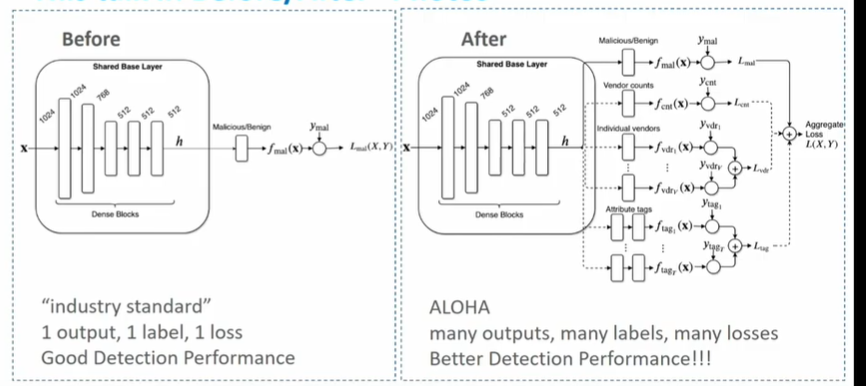
\includegraphics[width=9.5cm,height=10.5cm,keepaspectratio]{comparison arch.png}}
\caption{A Comparison between ALOHA Models and Industrial Standards }
\label{fig}
\end{figure}
The Auxiliary Loss Optimization Model for Hypothesis Augmentation uses Auxiliary inputs to optimize the weights of the network by adding more labels and reducing the search space to a more optimal one. The weights are fine tuned due to access to metadata during training. These auxiliary labels are then dropped at validation and deployment stage once the model is trained. 
The loss functions are denoted by L\textsubscript{loss type}(X,Y) for some input features X and targets Y – associated with the various outputs of the model, as well as how the labels Y representing the targets of these outputs are constructed. 
\begin{figure}[!h]
\centerline{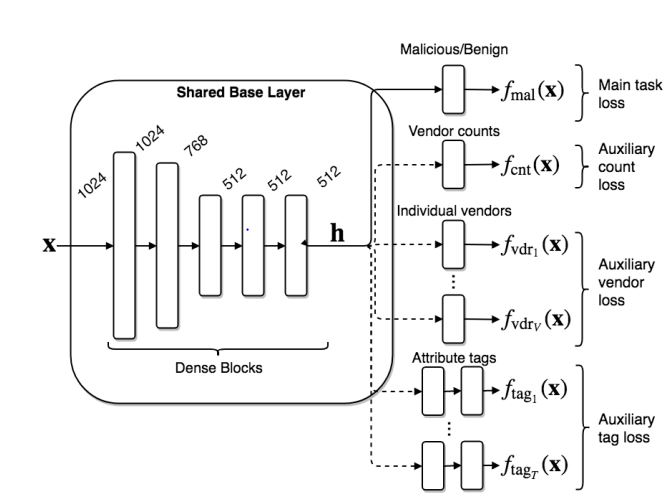
\includegraphics[width=9.5cm,height=10.5cm,keepaspectratio]{aloha.JPG}}
\caption{ALOHA Architecture }
\label{fig}
\end{figure}


In this model, multiple output layers with corresponding loss functions are optionally connected to a common base topology which consists of five dense blocks. The base model is a feedforward neural network. Each block in the network is composed of a Dropout, dense and batch normalization layers followed by an exponential linear unit (ELU) activation of sizes 1024, 768, 512, 512, and 512. This base, connected to our main malicious/benign output (solid line in the figure) with a loss on the aggregate label constitutes our baseline architecture. Auxiliary outputs and their respective losses are represented in dashed lines. When we deploy the model, the auxiliary outputs can be dropped. Hence, they are denoted by a dotted line in the figure.

The baseline for validations in the architecture is malicious and benign. To that auxiliary outputs are added with the structure as described above.

The auxiliary losses are of three types:
\begin{itemize}
    \item Count Loss
    \item Multi-label Vendor Loss
    \item  Multi-label Attribute Tag Loss
\end{itemize}
\subsubsection{Count Loss}
The count loss is given by:
\begin{equation}
  \label{eq:count_loss}
  L_{mal}(X,Y) = -\frac{1}{M} \sum^{M}_{i=1} \hat{y}^{(i)}\log{\hat{y}^{(i)}}+(1-\hat{y}^{(i)})\log(1-\hat{y}^{(i)})
\end{equation}

\subsubsection{Vendor Count Loss}
This is also called as Poisson count loss as the model can be approximated into a simpler function by assuming that the data follows Poisson Process.\cite{b3}
\begin{equation}
  \label{eq:vendor_count_loss}
  L_{p}(X,Y) = \frac{1}{M} \sum^{M}_{i=1} \mu^{(i)}-\hat{y}^{(i)}\log{(\mu^{(i)})} + \log{(\hat{y}^{(i)}!)} 
\end{equation}
\subsubsection{ Per-Vendor Malware Loss}
\begin{equation}
  \label{eq:per_vendor_malware_loss}
  L_{p}(X,Y) = \frac{1}{M} \sum^{M}_{i=1} \mu^{(i)}-\hat{y}^{(i)}\log{(\mu^{(i)})} + \log{(\hat{y}^{(i)}!)} 
\end{equation}

\subsubsection{Malicious Tags Loss}
\begin{equation}
  \label{eq:malicious_tag_loss}
  L_{p}(X,Y) = \frac{1}{M} \sum^{M}_{i=1}\sum^{T}_{i=1} l_{tag}(f_{tag_{j}}(x^{i}),{y_{t_{j}}}^{(i)}) 
\end{equation}
Plugging in the necessary functions, we get 
\begin{equation}
  \label{eq:malicious_tag_loss_long}
  L_{vdr}(X,Y)=-\frac{1}{M} \sum^{M}_{i=1}\sum^{T}_{j=1}\hat{y_{t_{j}}}^{(i)}\log{(\hat{y_{t_{j}}}^{(i)})}+(1-\hat{y_{t_{j}}}^{(i)})\log(1-\hat{y_{t_{j}}}^{(i)})
\end{equation}
\cite{b1}

\subsection{Broad Classification of Domain Generation Algorithms}
Based on reviewing multiple sources(\cite{b3} \cite{b9}\cite{b11}), we can come up with the following broad scaled classification of Domain Generation Algorithms[It is important to note that different sources classify the same algorithm into different classes]:
\begin{itemize}
\item \textbf{Classical Domain Generation Algorithms} : The general methodology used by a Classical Domain Generation Algorithm is using a deterministic pseudo-random generator (PRNG) to generate a list of candidate domain names. The seed of a PRNG can be the current date, some magic numbers, an exchange rate, etc. This random generator can be a single uniform distribution generator to generate a string sequence as the domain name (Example: Conficker, Ramnit, and others). 
Figure 3 shows an example of how a classical Domain Generation Algorithm algorithm workflow typically looks like.
\begin{figure}[!h]
\centerline{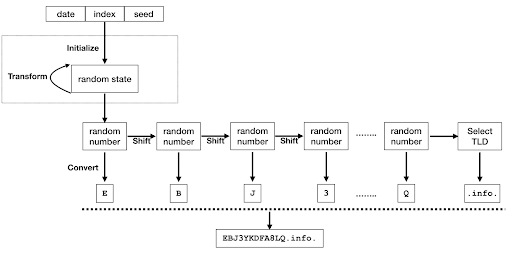
\includegraphics[width=9.5cm,height=14.5cm,keepaspectratio]{classic-DGA.png}}
\caption{Classical DGA Architecture }
\label{fig}

\end{figure}

\item \textbf{Word Based Domain Generation Algorithms} : These algorithms use english words as seeds to generate domain names. As a result, the domain name consists of english words but is still a malware.
\item \textbf{High collision Domain Generation Algorithms} : Domain names generated using this Domain Generation Algorithm are harder to detect as it generates Domains very similar to actual domain names.Example Domain Generation Algorithm algorithms which belong to this class is Virut.
\end{itemize}


\section{Proposed Solution}

\subsection{ALOHA for Algorithmically Generated Domain Names}
Our goal is to develop a model that can fit well into the traditional architectures structure used in the industry while it is deployed. Thus, the implementation is based on ensuring that while the model receives input it can also be deployed to an actual network if needed.
Following are the key features of the model:
\begin{itemize}
\item The model has two states: Training state and Validation state. 
\item We are using auxiliary inputs at the time of training to reduce and optimize the possible search space to get more accurate results. This is done by fine tuning the weights across multiple layers in the model.
\item According to the original paper any accuracy gains observed by the model is due to the correlation effect. The weights of the model are “fine-tuned” by using meta data(Auxiliary Labels). When it is deployed we can remove the extra labels.
\item The domain names are generated by using standard open-source implementations of certain common DGAs listed in the results section.
\end{itemize}
\cite{b3}
\subsubsection{Loss Equation for the ALOHA DGA Models}
\begin{equation}
  \label{eq:malicious_tag_loss}
  L = L_1+\sum_{{i\in DGA}}\lambda L_2i
\end{equation}
Where $L_1$ and $L_2i$ are binary cross entropy loss functions and $\lambda = 1$. DGA refers to the class to which the giving domain generated belongs to. For our model:\\
  $DGA$ = \{$banjori$, $corebot$, $cryptolocker$, $dircrypt$, $kraken$,\\ $lockyv2$, $qakbot$, $ramdo$, $ramnit$, $simda$, $gozi$,\\ $suppobox$, $matsnu$, $pykspa$ \}

\subsection{Key issues with the proposed model}
\begin{itemize}
\item \textbf{Hard to find relevant and organized sources of Meta-Data}: Sources of meta-data are scattered. As we feed more and more meta-data the model should give improved results. As of now we don’t have enough structured meta-data. The first objective was to review the multiple sources which could be used for metadata generation.
\item \textbf{Classification of Domain Generation Algorithms}: I was unable to find a single review paper that could list down all the common classes of review paper. After collating information from multiple sources, I have identified some of the most popular classes of Domain Generation Algorithms.
\item \textbf{The Problem of Non Domain Generation Algorithms} :  There are certain domain names which can be generated by DGA algorithms which are actual domain names instead of bogus domain names. The model needs to recognise these domain names to be domains that exist instead of being an algorithmically generated domain name. Hence, achieving a 100\% accuracy is difficult.
\end{itemize}
\subsection{Potential Sources of Metadata/Auxiliary Labels}
Below are listed some potential sources of metadata(auxiliary targets) gathered based on literature review and discussions during project meets:
\begin{itemize}
\item Data generated or gathered from passive DNS:
\textbf{Datasets Found}: 
\begin{itemize}
\item DGArchive\cite{b12}
\end{itemize}
However, it is possible to generate a passive DNS dataset over multiple weeks. There are research papers and theses that have used this method and explain the procedure.\cite{b10}
\item \textbf{Virus Total's Domain Report} has some data related to domain names. 
\item Information related to the domain name and how it is generate like the type of DGA(alphanumeric, hex-based, word-based).
\item \textbf{Classical DGA features} like string entropy,count of the longest consecutive vowel/consonant string can be used as auxiliary inputs.
\item  We can use certain \textbf{cryptographic measures like index of coincidence} as meta data for a given domain name. This can be a particularly insightful source of meta data for word based DGAs. \\
For x = (x\textsubscript{1},x\textsubscript{2},...,x\textsubscript{n}) which is a string of the english alphabet.\\
I\textsubscript{c}(x) is the probability that two random elements of x are identical. Let f\textsubscript{1},f\textsubscript{2},...,f\textsubscript{26} be the number of occurrences of letters A,B,...,Z in the string x then
\begin{equation}
      \label{eq:index_of_coincidence}
  I_{c}(x) = \frac{\sum^{25}_{i=1} \binom{f_{i}}{x}}{\binom{n}{2}} 
\end{equation}
\end{itemize}
\subsection{Architecture Details}
We used the following baseline architectures:
\begin{itemize}
\item Bigram
\item LSTM \cite{b6}
\item CNN   \cite{b7}
\item LSTM + CNN \cite{b6,b7}
\end{itemize}
The corresponding ALOHA Architectures are as follows:
\begin{itemize}
\item ALOHA CNN
\item ALOHA Bigram
\item ALOHA LSTM
\item ALOHA CNN+LSTM
\end{itemize}
\subsection{Implementation Details\cite{b13}}
\begin{itemize}
\item \textbf{Source of Metadata Used in the project}: The current implementation uses the malware family[Example: Banjori, Pykspa] as auxiliary input. To use a certain dataset the data must be easy to organise systematically. Hence, we only only choose certain kinds of auxiliary labels for our model.
\item \textbf{Dataset Generation Methods}: The implementation is based on the open source implementation by Endgame Inc.\cite{b7}

\item \textbf{Parameter Details}:
For avoiding training a bias due to the Top level domain all the DGAs have been stripped of the Top level Domain. While training and validation the model does not take the top level domain into consideration.
For implementing the ALOHA model for Algorithmically Generated Domain Names we set the weights of the auxiliary labels to 0.1 and the weight of the primary label to 1.\cite{b5}\\
The list of parameters used in the model and their values are as follows:

\begin{itemize}
\item Name of the class of algorithm used to produce the domain name: It is the malware family that the given algorithm belongs to.The weight assigned is 0.1.
\item Main Target: Weight assigned is 1.
\end{itemize} 
\item \textbf{Dataset Split}: 76\% Training set, 4\% Validation set and 20\% Testing Set 
\item \textbf{Experimental Setup}: We run two experiments. First we train and validate the model for all DGAs mentioned above. Further, we train and validate the model only on Word Based DGAs to verify our hypothesis that ALOHA provides improved results for certain Deep Learning Architectures in case of Word Based Domain Generation Algorithms.  

\end{itemize}
\section{Experimental Results}
\subsection{Dataset Details}\label{AA}
\subsubsection{Analysis of Alexa Top 1million Domain names and the DGA Domain Names Used for training the Model}
The count of how many domains generated by each DGA family were used and how many Alexa top 1m domains[listed as benign] were included:
\begin{itemize}
\item ('benign', 139935)
\item ('corebot', 10000)
\item ('dircrypt', 10000)
\item ('kraken', 10000)
\item ('pykspa', 10000)
\item ('qakbot', 10000)
\item ('ramnit', 10000)
\item ('matsnu', 10000)
\item ('suppobox', 10000)
\item ('gozi', 10000)
\item ('locky', 9999)
\item ('banjori', 9984)
\item ('cryptolocker', 9984)
\item ('ramdo', 9984)
\item ('simda', 9984)
\end{itemize}
Note: The tupled format indicates the number of domain names which are generated using the corresponding class of algorithms. Benign indicates actual domains which are obtained from the Alexa top 1m domains dataset.
\subsubsection{Classification of the DGAs Used in the model}
\begin{itemize}
\item \textbf{Classical DGAs}: banjori, corebot, cryptolocker, dircrypt, kraken, lockyv2, qakbot, ramdo, ramnit, and simda.
\item \textbf{Word-based/dictionary DGAs} - gozi, suppobox, matsnu and pykspa 
\end{itemize}
\section{Case-wise Result Summary}
\subsection{Case 1}
\textbf{Classical as well as word-based and other non-classical algorithms are not differentiated.}
\subsubsection{Consolidated Graphs}
Refer Fig 4 and Fig 5 \\
\begin{figure}[!h]
\centerline{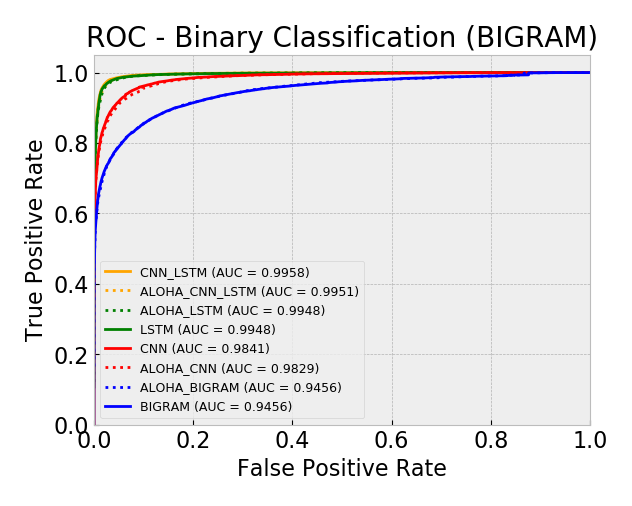
\includegraphics[width=9.5cm,height=10.5cm,keepaspectratio]{linear_scale_all_dga.png}}
\caption{Linear Scale Summary for All DGAs }
\label{fig}

\centerline{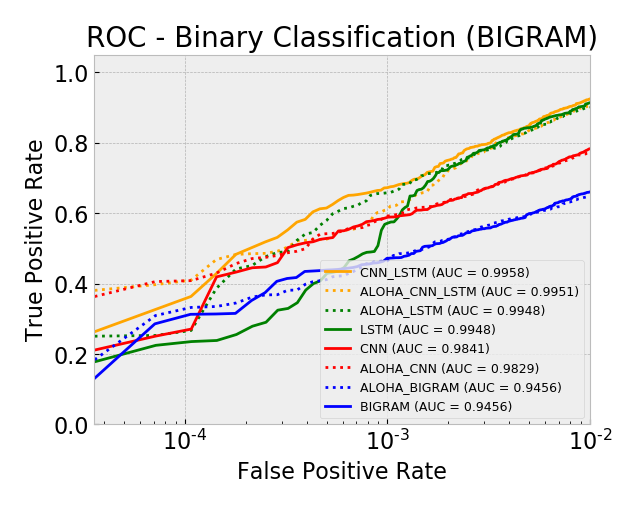
\includegraphics[width=9.5cm,height=10.5cm,keepaspectratio]{log_scale_all_dga.png}}
\caption{Logarithmic Scale Summary for All DGAs }
\label{fig}
\end{figure}

\subsubsection{Analysis for Individual Domain Generation Algorithms} 
Refer Fig 6\\
\begin{figure}[!h]
\centerline{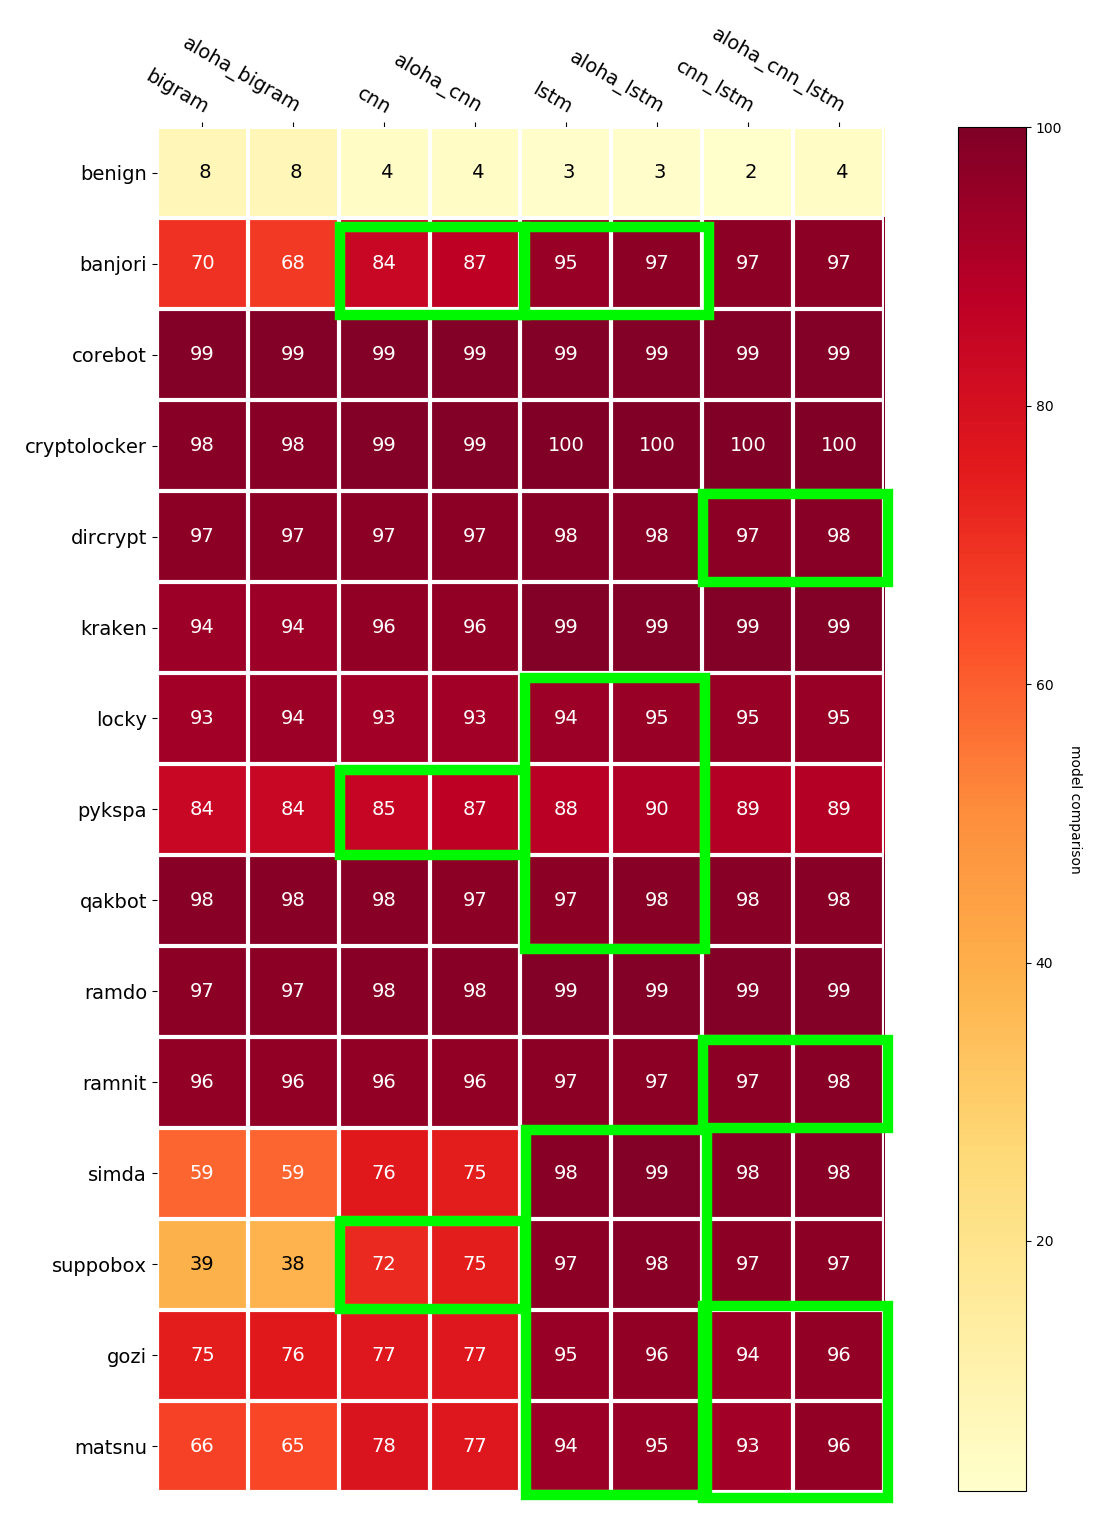
\includegraphics[width=9.5cm,height=10.5cm,keepaspectratio]{heatmap.png}}
\caption{Heatmap with Accuracy Calculated for All DGAs  }
\label{fig}
\end{figure}

\subsection{Case 2}
\textbf{ALOHA on Word Based DGAs Only}
\subsubsection{Consolidated Graphs}
Refer Fig 7 and Fig 8\\
\begin{figure}[!h]
\centerline{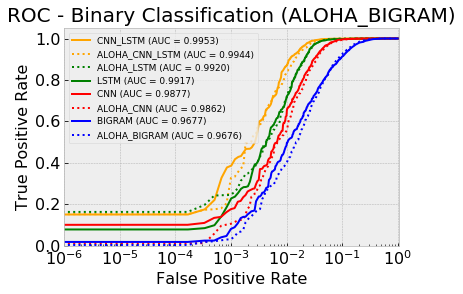
\includegraphics[width=9.5cm,height=13.5cm,keepaspectratio]{linear_scale_word_dga.png}}
\caption{Linear Scale Summary for Word Based DGAs }
\label{fig}
\centerline{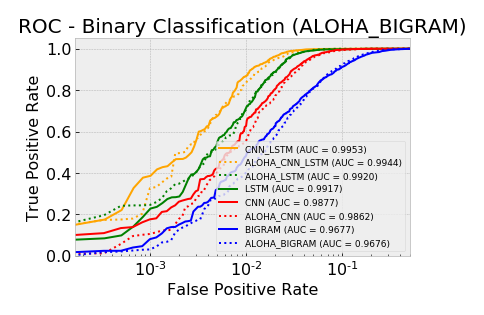
\includegraphics[width=9.5cm,height=13.5cm,keepaspectratio]{logscale_word_dga.png}}
\caption{Logarithmic Scale Summary for Word Based DGAs }
\label{fig}
\end{figure}


\subsubsection{Analysis for Individual Word Based Domain Generation Algorithms}
Refer Fig 9 \\
\begin{figure}[!h]
\centerline{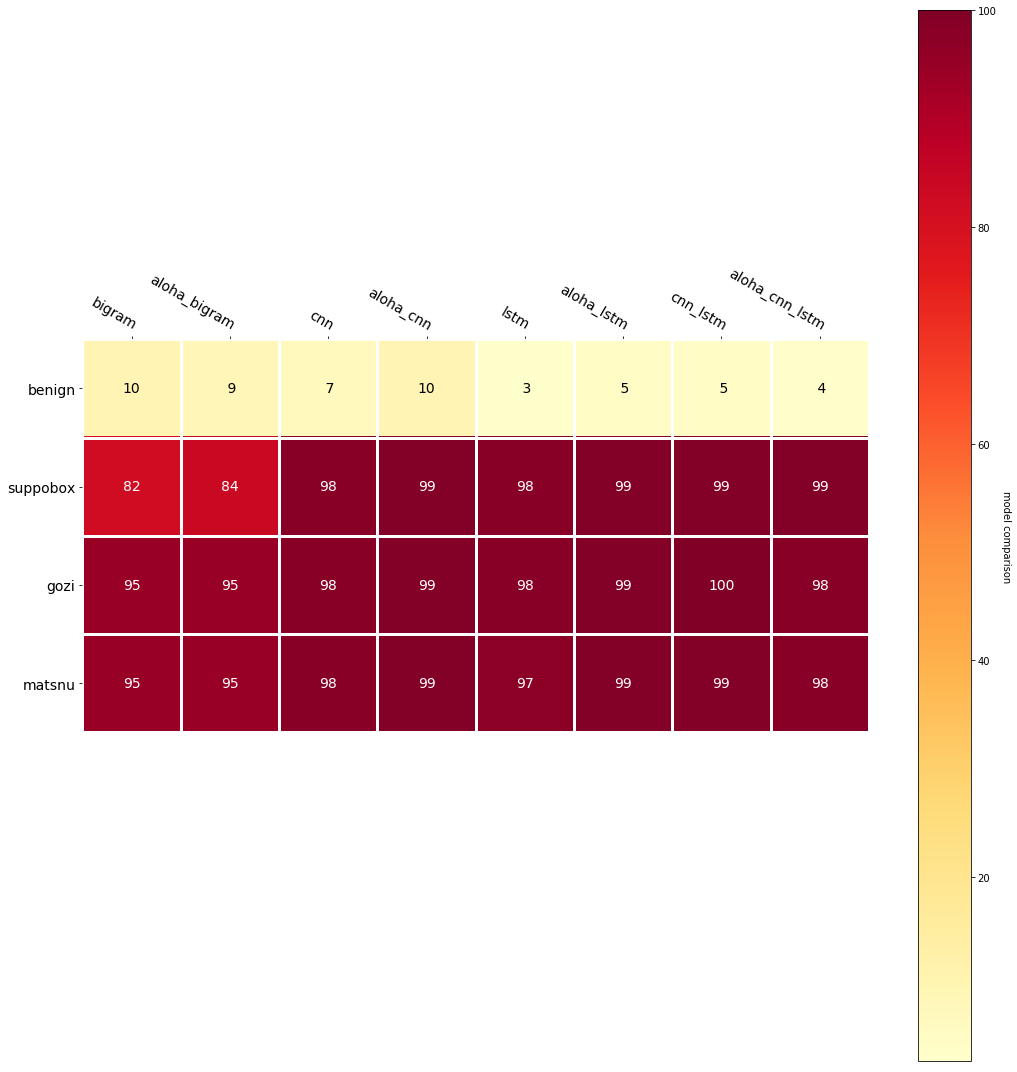
\includegraphics[width=7.5cm,height=10.5cm,keepaspectratio]{heatmap_word.png}}
\caption{Heatmap with Accuracy Calculated for Word Based DGAs  }
\label{fig}
\end{figure}


\subsection{Case 3}
\textbf{ALOHA on High Collision DGA}
\subsubsection{Consolidated Graphs}
Refer Fig 4 and Fig 5\\
\begin{figure}[!h]
\centerline{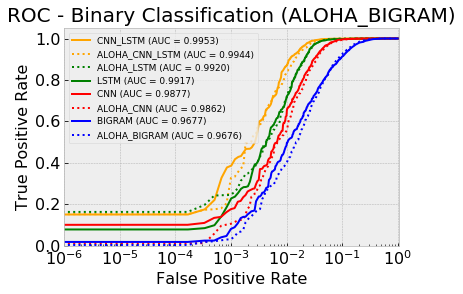
\includegraphics[width=9.5cm,height=13.5cm,keepaspectratio]{linear_scale_word_dga.png}}
\caption{Linear Scale Summary for Word Based DGAs }
\label{fig}
\centerline{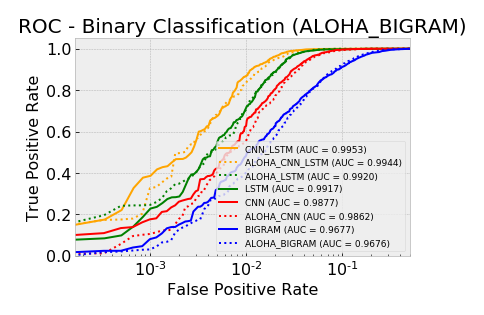
\includegraphics[width=9.5cm,height=13.5cm,keepaspectratio]{logscale_word_dga.png}}
\caption{Logarithmic Scale Summary for Word Based DGAs }
\label{fig}
\end{figure}


\subsubsection{Analysis for Individual Word Based Domain Generation Algorithms}
Refer Fig 6 \\
\begin{figure}[!h]
\centerline{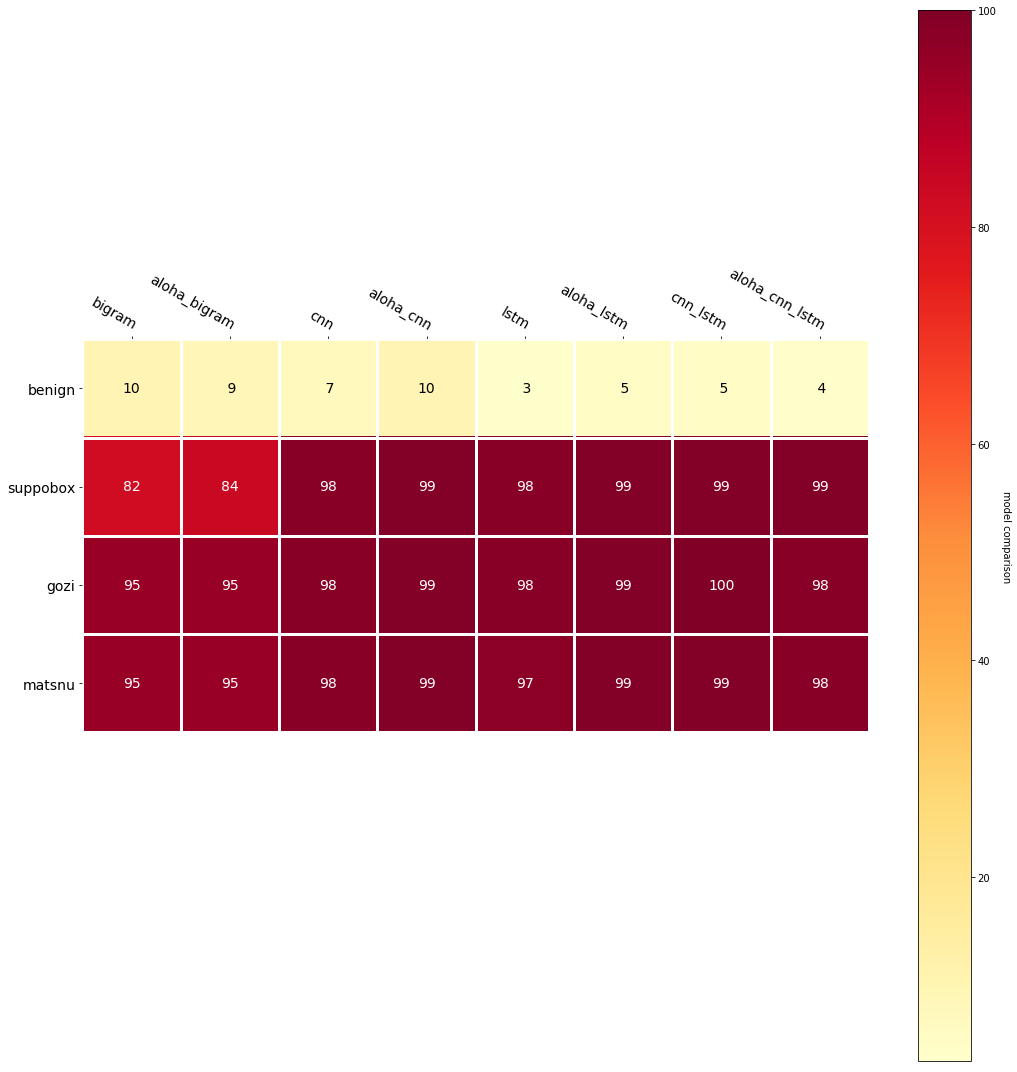
\includegraphics[width=7.5cm,height=10.5cm,keepaspectratio]{heatmap_word.png}}
\caption{Heatmap with Accuracy Calculated for Word Based DGAs  }
\label{fig}
\end{figure}



\section{Conclusion}
\subsection{Case 1:No Differentiation}
In general, for all algorithms ALOHA does not give a lot of improvement. In fact, in some cases, it is observed that a baseline model performs better than the ALOHA model. We observe that in case of LSTM models in word based DGAs there is a significant improvement if we use ALOHA. But this does not happen in other standard deep learning architectures. The results could be improved by adding more auxiliary inputs to the model. 

\subsection{Case 2:Word Based DGAs}
It is observed that ALOHA gives some improvement for Word Based Domain Generation Algorithms, particularly for the LSTM architecture. The results can be improved further by adding more data inputs in the future. 
\section{Further Work}
The model should be expanded to include more commonly used Word Based Domain Generation Algorithms like nymaim2(word based version of nymaim) and pizd. The results need to be thoroughly verified for the same before drawing any conclusions. One could also test the model on generalized standard DGA datasets like DGArchive. The implementation must be modified to suit the needs of the dataset being used for training. But, in general the conclusions would remain the same.
\section*{Acknowledgment}
I would like to thank BITS Pilani for providing me an opportunity to take up this Laboratory
Oriented Project. I want to thank my guide, Dr. Ashutosh Bhatia for his guidance and inputs that helped me handle all the obstacles with considerable ease.


% \bibliography{sample}
% \bibliographystyle{IEEEtran}


\section{References}
\begin{thebibliography}{00}
\bibitem{b1} ALOHA: Auxiliary Loss Optimization for Hypothesis Augmentation[ arXiv:1903.05700 [cs.CR] ]
\bibitem{b2} Detecting DGA domains with recurrent neural networks and side information
\bibitem{b3} Botnet Detection Using Passive DNS (Master Thesis by Pedro Marques da Luz)
\bibitem{b4} \url{https://conferences.sigcomm.org/sigcomm/2015/pdf/papers/p91.pdf}
\bibitem{b5} \url{http://www.covert.io/}
\bibitem{b6} \url{https://github.com/keeganhines/snowman}[Used for implementing LSTM based baseline architectures]
\bibitem{b7} \url{https://github.com/endgameinc/dga_predict} [ Used for implementing CNN baseline model]
\bibitem{b8} \url{https://arxiv.org/pdf/1811.08705.pdf}
\bibitem{b9} \url{https://blogs.akamai.com/2018/01/a-death-match-of-domain-generation-algorithms.html}
\bibitem{b10} The Internet of Names: A DNS Big Dataset URL:\url{https://conferences.sigcomm.org/sigcomm/2015/pdf/papers/p91.pdf}
\bibitem{b11}  Sood, A. K., & Zeadally, S. (2016). A Taxonomy of Domain-Generation Algorithms. IEEE Security & Privacy, 14(4), 46–53. doi:10.1109/msp.2016.76
\bibitem{b12} \url{https://dgarchive.caad.fkie.fraunhofer.de/site/}
\bibitem{b13}\url{https://github.com/ighosh98/DGA-Prediction} [Code Implementation for the Project ]
\end{thebibliography}
\vspace{12pt}

\end{document}
